\section{Результаты проведённого анализа}

Цель данного раздела настоящей работы \--- сравнение решений обыкновенного дифференциального уравнения с запаздыванием

\begin{equation}\label{eq:result-ODE-delay}
{T'}_{k}(t) - \gamma(k^2) T_k(t-\tau)=0
\end{equation}

и его приближений обыкновенными дифференциальными уравнениями уже без запаздывания:

\begin{equation}\label{eq:result-ODE-no-delay}
\sum\limits_{n=1}^{m} \dfrac{\tau^{n-1}}{(n-1)!} T_k^{(n)} (t) + \gamma(k^2) T_k (t) = 0
\end{equation}

В предыдущих главах было доказано, что достаточным условием устойчивости (\ref{eq:result-ODE-delay}) является соотношение $\gamma \tau <1$. Приближения (\ref{eq:result-ODE-no-delay}) же, вообще говоря, всегда неустойчивы при порядках $m \geq 6$ и неустойчивы в предположениях фиксированного малого $\tau$ для порядков $m \geq 2$. Приближение порядка $m=1$ всегда устойчиво.

В рамках работы была написана программа для построения графиков решений задач Коши для функций (\ref{eq:result-ODE-delay}) и (\ref{eq:result-ODE-no-delay}) в зависимости от параметров 

\begin{enumerate}
\item $\tau$ \--- величины запаздывания,
\item $k$ \--- порядка члена ряда Фурье,
\item $m$ \--- порядка приближения.
\end{enumerate}

Начальной функцией предполагается единичная функция на $[-\tau,0]$. Скорости $a$ и $v$ для простоты примем также единичными.

Будем обозначать как $T$ \- решение (\ref{eq:result-ODE-delay}) и как $Tm$ \--- решение \ref{eq:result-ODE-no-delay}.

\newpage

\subsection{Графики решений при $\tau=0.1$, $k=1$}

\vfill

\begin{figure}[h]
\begin{center}
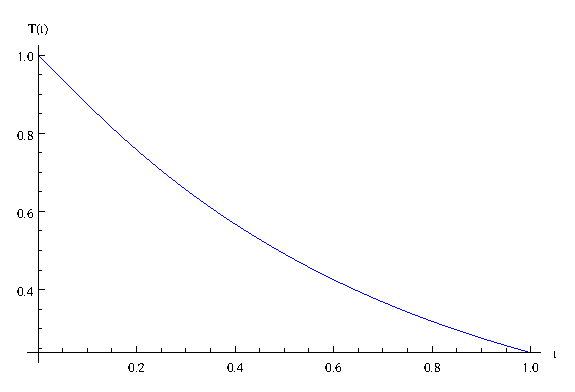
\includegraphics[width=0.9\textwidth]{./3_results/1_1.eps}
\end{center}
\caption{График для $T(t)$ при $\tau=0.1$, $k=1$, $m=1$}
\end{figure}

\vfill

\newpage

\subsubsection{Приближение порядка $m=1$}

\begin{figure}[h]
\begin{center}
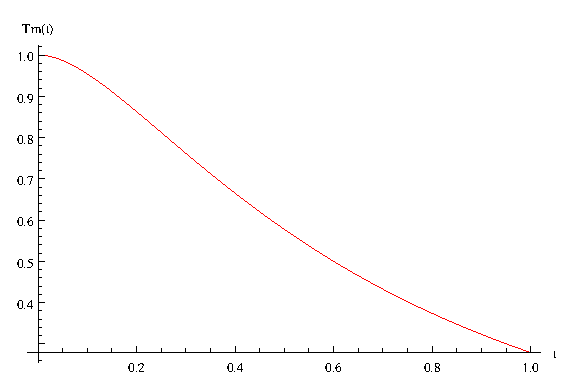
\includegraphics[width=0.65\textwidth]{./3_results/1_2.eps}
\end{center}
\caption{График для $Tm(t)$ при $\tau=0.1$, $k=1$, $m=1$}
\end{figure}

\begin{figure}[h]
\begin{center}
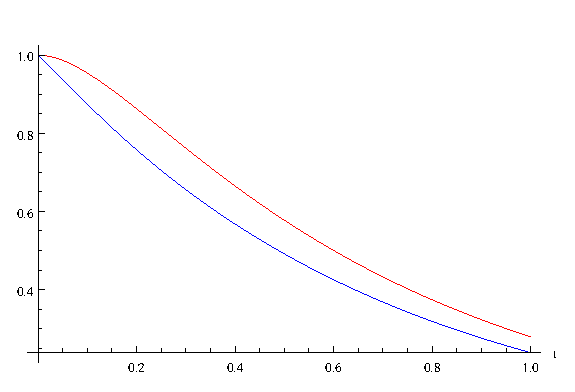
\includegraphics[width=0.65\textwidth]{./3_results/1_3.eps}
\end{center}
\caption{Общий график при $\tau=0.1$, $k=1$, $m=1$}
\end{figure}